\chapter{Polynomial Approximations - Interpolation}
% Brady is currently working on this section

The reason people have such interest in polynomials---and in polygons and polyhedra---is because of the following approximation theorem:

\begin{theorem}[Weierstrass Approximation Theorem]
If $f$ is any continuous function on the finite closed interval $[a,b]$, then for every $\epsilon>0$ there exists a polynomial $p(x)$ (whose degree and coefficients depend on $\epsilon$) such that 
$$
\max_{x\in [a,b]} \mid f(x) - p(x) \mid \; < \, \epsilon
$$
\end{theorem}

Of course, this theorem doesn't tell us how to construct $p(x)$, or even what the degree of $p(x)$ is. \\

We will look at the construction of interpolating polynomials, at error estimates, and some difficulties.
In practice, one patches together series of low-order polynomial approximations, such as in splines and Bezier patches.

\subsection*{Applications}
\begin{itemize}
    \item Modeling scenes with sparse data.
    \item CAD representations.
    \item Data compression. (e.g., tables)
    \item Generating robot trajectories that pass through given set points (inverse kinematics). 
\end{itemize}

\section{Polynomial Forms}

\textbf{Power form:}
$$
p(x) = a_0 + a_1 x + a_2 x^2 + \dots + a_n x^n
$$
where $a_n \neq 0$ and the polynomial is degree $n$. Numerical round-off can lead to a loss of significance for $x$ no near zero. \\

\textbf{Shifted power form:}
$$
p(x) = a_0 + a_1 (x-c) + a_2 (x-c)^2 + \dots + a_n(x-c)^n
$$

Taylor expansion for $p(x)$ about $c$ and $a_i = \frac{p^{(i)}(c)}{i!}$

\textbf{Newton form:}
\begin{align}
p(x) = a_0 &+ a_1 (x-c_1) \\
           &+ a_2 (x-c_1)(x-c_2) \\
           &\,+ \\
           &\,\, \vdots \\
           &\,+ \\
           &a_n (x-c_1)(x-c_2)\dots(x-c_n)
\end{align}
$n+\frac{n(n+1)}{2}$ adds; $\frac{n(n+1)}{2}$ multiplies.

\textbf{Nested Newton form:}
$$
p(x) = a_0 + (x-c_1)\left\{a_1 + (x-c_2)\left[a_2 + \dots + (x-c_{n-1})(a_{n-1}+(x-c_n)a_n)\right]\right\}
$$
$2n$ adds; $n$ multiplies. \\

It is easy to write a recursive algorithm to evaluate $p(x)$ in nested Newton form. To evaluate $p(x)$ given $x$, $a_0, \dots, a_n$, $c_1, \dots, c_n$: \\

\quad \textsf{poly\_eval}($x$; $a_0, \dots, a_n$; $c_1, \dots, c_n$)

\qquad \qquad $a_0 + (x-c_1)\cdot $\textsf{poly\_eval}($x$; $a_1, \dots, a_n$; $c_2, \dots, c_n$)

\section{Polynomial Interpolation}

Suppose $f: [a,b] \rightarrow \mathbb{R}$ \\

And suppose $x_0, x_1, \dots , x_n$ are $n+1$ distinct points in $[a,b]$. \\

\noindent We want to construct a polynomial of degree $n$ or less that interpolates $f(x)$ at the points $\{x_i\}$. 
That is, we want a polynomial $p(x)$ such at

\begin{equation*}
    p(x_i) = f(x_i) \qquad i = 1, \dots, n.
\end{equation*}

There exists a unique such polynomial. We will see it shortly. \\

To see uniqueness, suppose $p$ and $q$ are each polynomials of degree at most $n$ that agree at the $\{x_i\}$. 
Then $p-q$ is a polynomial of degree at most $n$ that vanishes at the $\{x_i\}$. 
Therefore, by the Fundamental Theorem of Algebra

\begin{equation*}
    (p-q)(x) = c \prod_{i=0}^n (x-x_i)
\end{equation*}
where $c$ is some real number. The left hand side has degree at most $n$. The right hand side has degree exactly $n+1$, unless $c=0$. So, $c=0$, and then $p=q$, meaning that $p$ is unique. \\

Uniqueness tells us that the different ways of writing the interpolating polynomial $p(x)$ are really the same, and must therefore differ primarily on numerical grounds (e.g. compactness, stability, ...). \\

\subsection{Lagrange Form}

The \underline{Lagrange Form} is a straightforward way of constructing the interpolating polynomial:

\begin{equation*}
    p(x) = a_0 l_0 (x) + a_1 l_1 (x) + \dots + a_n l_n (x)
\end{equation*}
where each $l_i(x)$ is a polynomial of degree $n$ that satisfies
\begin{equation*}
    l_i(x_k) = \begin{cases}
      1 \quad \mathrm{if} \quad i=k\\
      0 \quad \mathrm{if} \quad i \neq k
    \end{cases}  
\end{equation*}
$i=0,\dots,n$ and $a_i=f(x_i)$. \\

In other words,
\begin{equation*}
    l_i(x) = \prod_{\substack{k=0 \\ k\neq i}}^n \frac{x-x_k}{x_i-x_k}
\end{equation*}

\underline{Ex} Suppose we start with a polynomial, say 
\begin{equation*}
    f(x) = (x-1)^2
\end{equation*}
And suppose we have two values, at $x_0=0$ and $x_1 = 1$:

\begin{equation*}
    \begin{split}
        f(0)=1 \quad \Rightarrow \quad a_0 = 1 \\
        f(1)=0 \quad \Rightarrow \quad a_1 = 0
    \end{split}
\end{equation*}
Now $p(x) = a_0 l_0 (x) + a_1 l_1 (x)$ \\

Since $a_1 = 0$, we only care about $l_0(x)$.

\begin{equation*}
    l_0 (x) = \frac{x-x_1}{x_0-x_1} = \frac{x-1}{0-1} = -x + 1
\end{equation*}
so $p(x) = -x + 1$, which is a line. \\

This polynomial interpolates $f(x)$, but not very well, as one would imagine.

\begin{figure}[H]
    \centering
    % \includegraphics[width=0.8\textwidth]{figures/chap_03/polynomial-1.png}
    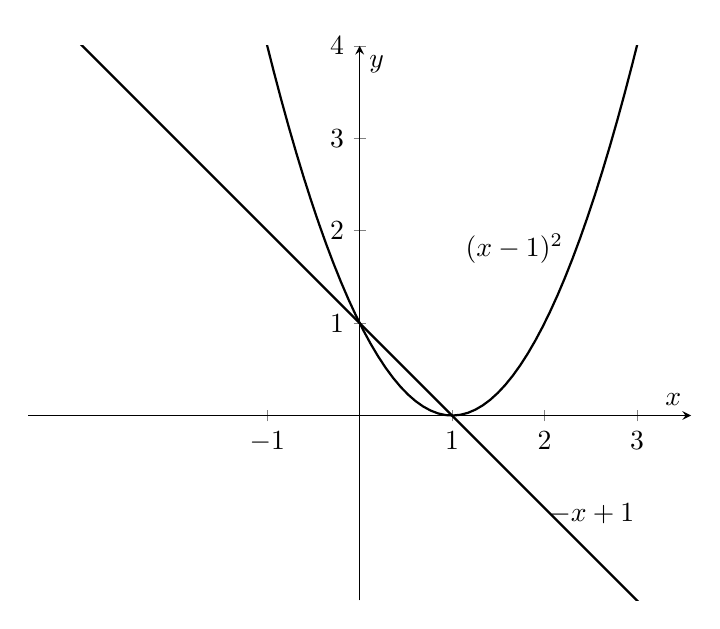
\begin{tikzpicture}
\begin{axis}[
axis y line=center,
axis x line=middle,
axis equal,
xmax=3,xmin=-3,
ymin=-2,ymax=4,
xlabel=$x$,ylabel=$y$,
xtick={-1,0,1,2,3},
ytick={1,2,3,4},
width=10cm,
samples=100,
anchor=center,
]
\addplot[thick,domain=-4:4,mark=none]{(x-1)^2} node[yshift=1cm,pos=0.75, above, label={$(x-1)^2$}] {};
\addplot[thick,domain=-4:4,mark=none]{-x+1} node[pos=0.8, right, label={$-x+1$}] {};
\end{axis}
\end{tikzpicture}

    % \caption{Caption}
    \label{fig:polynomial-1}
\end{figure}
So, let's add the value of $f$ at a third point, say $x=-1$. 

\subsection{Divided Differences}

\subsection{Error of the interpolating polynomial}

\begin{figure}
  \centering
  \label{}
  \caption{}
  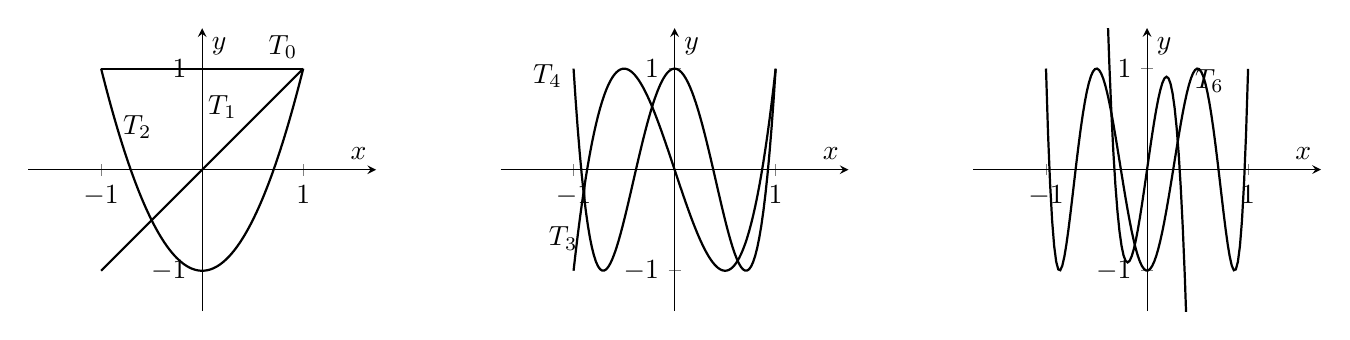
\begin{tikzpicture}
\begin{axis}[
axis y line=center,
axis x line=middle,
axis equal,
xmax=1,xmin=-1,
ymin=-1.4,ymax=1.4,
xlabel=$x$,ylabel=$y$,
xtick={-1,+1},
ytick={-1,+1},
width=6cm,
samples=100,
anchor=center,
]
\addplot[thick,domain=-1:1,mark=none]{(1)} node[pos=0.9, below, label={$T_0$}] {};
\addplot[thick,domain=-1:1,mark=none]{x} node[pos=0.6, above, label={$T_1$}] {};
\addplot[thick,domain=-1:1,mark=none]{2*(x^2)-1} node[pos=0.2, right, label={$T_2$}] {};
\end{axis}
\begin{scope}[xshift=6cm]
\begin{axis}[
axis y line=center,
axis x line=middle,
axis equal,
xmax=1,xmin=-1,
ymin=-1.4,ymax=1.4,
xlabel=$x$,ylabel=$y$,
xtick={-1,0,1,2,3},
ytick={-1,1},
width=6cm,
samples=100,
anchor=center,
]
\addplot[thick,domain=-1:1,mark=none]{4*(x^3) - 3*x} node[pos=0.0, left, label={$T_3$}] {};
\addplot[thick,domain=-1:1,mark=none]{8*(x^4) - 8*(x^2) + 1} node[shift={(-0.2cm,-0.5cm)},pos=0.0, left, label={$T_4$}] {};
\end{axis}
\end{scope}

\begin{scope}[xshift=12cm]
\begin{axis}[
axis y line=center,
axis x line=middle,
axis equal,
xmax=1,xmin=-1,
ymin=-1.4,ymax=1.4,
xlabel=$x$,ylabel=$y$,
xtick={-1,0,1,2,3},
ytick={-1,1},
width=6cm,
samples=100,
anchor=center,
]
\addplot[thick,domain=-1:1,mark=none]{32*(x^6)-48*(x^4)+18*(x^2)-1} node[pos=0.7, below, label={$T_6$}] {};
\addplot[thick,domain=-1:1,mark=none]{64*(x^7) - 112*(x^5)-56*(x^3)+7*x} node[pos=0.7, below, label={$T_7$}] {};
\end{axis}
\end{scope}
\end{tikzpicture}

\end{figure}
\begin{figure}
  \centering
  \label{}
  \caption{}
  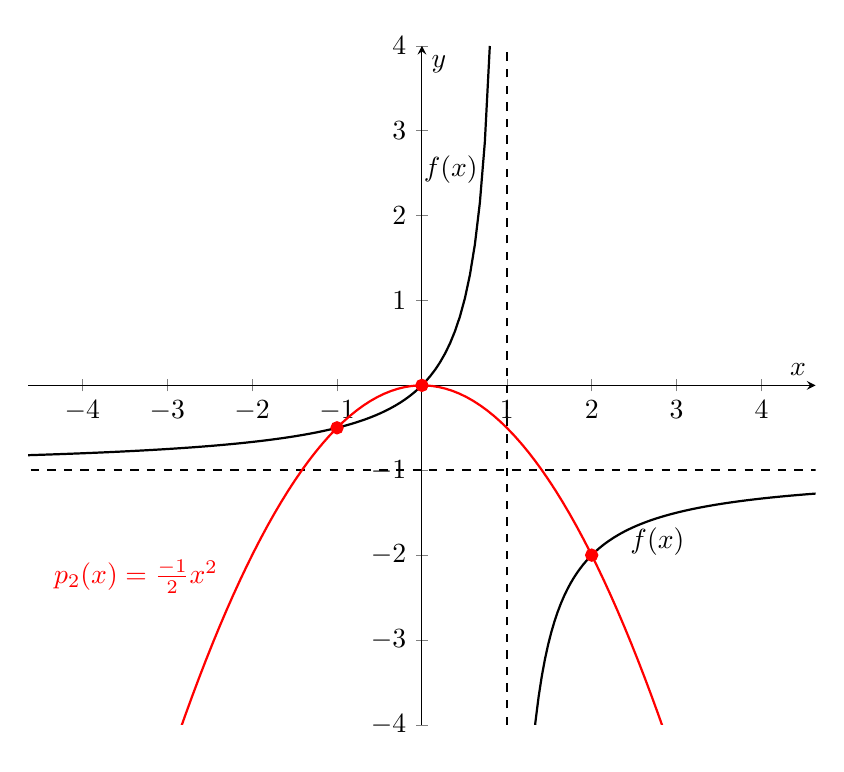
\begin{tikzpicture}
\begin{axis}[
axis y line=center,
axis x line=middle,
scale only axis,
axis equal,
xmax=3,xmin=-3,
ymin=-4,ymax=4,
xlabel=$x$,ylabel=$y$,
width=10cm,
samples=100,
anchor=center,
]
\addplot[thick,domain=-5:0.8,mark=none]{x/(1-x)} node[xshift=-0.5cm,pos=0.8, right, label={$f(x)$}] {};
\addplot[thick,domain=1.3:5,mark=none]{x/(1-x)} node[yshift=-0.6cm,pos=0.6, below, label={$f(x)$}] {};
;
\addplot[thick,mark=none,dashed] coordinates {(1, -4) (1, 4)};
\addplot[thick,mark=none,dashed] {-1};
\addplot[thick,domain=-4:4,red,mark=none] {-(x^2)/2} node[xshift=-1cm,pos=0.3, left, label={$p_2(x) = {-1 \over 2} x^2$}]{};
\addplot[thick,red,only marks] coordinates {(-1,-1/2) (0,0) (2,-2)};
\end{axis}
\end{tikzpicture}

\end{figure}
